\documentclass{beamer}
\mode<presentation>

\usepackage{tikz}
\usetikzlibrary{arrows.meta}
\usetikzlibrary{fit}
\usetikzlibrary{positioning}
\usetikzlibrary{shapes.multipart}

\title{Stack Graphs}
\author{Douglas Creager}
\institute{GitHub}
\date{Strange Loop 2021}

\setbeamertemplate{navigation symbols}{}

\usepackage{minted}
\usemintedstyle{colorful}

\usepackage{fontspec}
\setsansfont{Arial}
\setmonofont[Scale=0.8]{Iosevka Term}

\definecolor{sgdef}  {RGB}{159,0,0}
\definecolor{sgpop}  {RGB}{230,142,131}
\definecolor{sgref}  {RGB}{0,134,67}
\definecolor{sgpush} {RGB}{131,216,173}
\definecolor{sgjump} {RGB}{161,64,140}

\begin{document}

\begin{frame}
    \titlepage
\end{frame}

\begin{frame}
    \begin{center}
        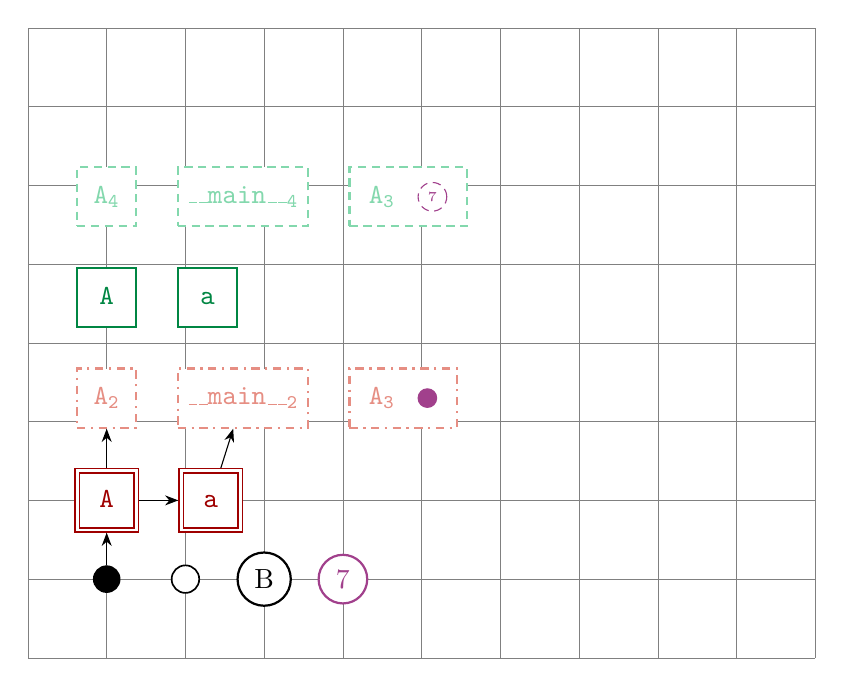
\begin{tikzpicture}
            \draw [help lines] (0,0) grid (10,8);

            % root
            \node (root)
              [circle, fill=black,
               inner sep=0pt, minimum size=0.35cm]
              at(1,1) {};

            % scope
            \node (s0)
              [circle, fill=white,
               draw=black, semithick,
               inner sep=0pt, minimum size=0.35cm]
              at(2,1) {};

            % named scope
            \node (sB)
              [circle, fill=white,
               draw=black, thick,
               minimum size=0.35cm]
              at(3,1) {B};

            % exported scope
            \node (s7)
              [circle, fill=white,
               draw=sgjump, thick,
               text=sgjump,
               minimum size=0.35cm]
              at(4,1) {7};

            % definitions
            \node (A)
              [fill=white,
               draw=sgdef, semithick, double, double distance=1pt,
               outer sep=1pt,
               text=sgdef,
               minimum size=0.75cm]
              at(1,2)
              {\texttt{\strut A}};
            \node (a)
              [right=0.5cm of A,
               fill=white,
               draw=sgdef, semithick, double, double distance=1pt,
               outer sep=1pt,
               text=sgdef,
               minimum size=0.75cm]
              {\texttt{\strut a}};

            % pop
            \node (A2)
              [above=0.5cm of A,
               fill=white,
               draw=sgpop, thick, dash dot,
               text=sgpop,
               minimum size=0.75cm]
              {\texttt{\strut A\textsubscript{2}}};
            \node (main2) 
              [right=0.5cm of A2,
               fill=white,
               draw=sgpop, thick, dash dot,
               text=sgpop,
               minimum size=0.75cm]
              {\texttt{\strut \_\_main\_\_\textsubscript{2}}};

            % pop scope
            \node (bar)
              [right=0.5cm of main2,
               rectangle split,
               rectangle split parts=2,
               rectangle split horizontal,
               rectangle split draw splits=false,
               rectangle split ignore empty parts,
               draw=sgpop, thick, dash dot,
               fill=white,
               text=sgpop,
               inner xsep=7pt,
               minimum size=0.75cm]
              {
                  \texttt{\strut A\textsubscript{3}}
                  \nodepart{two}
                  \hspace{-10pt}
                  \tikz \node [circle, fill=sgjump, inner sep=0pt, minimum size=0.25cm] {};
              };

            % references
            \node (A3)
              [above=0.5cm of A2,
               fill=white,
               draw=sgref, thick,
               text=sgref,
               minimum size=0.75cm]
              {\texttt{\strut A}};
            \node (a3)
              [right=0.5cm of A3,
               fill=white,
               draw=sgref, thick,
               text=sgref,
               minimum size=0.75cm]
              {\texttt{\strut a}};

            % push
            \node (A4)
              [above=0.5cm of A3,
               fill=white,
               draw=sgpush, thick, densely dashed,
               text=sgpush,
               minimum size=0.75cm]
              {\texttt{\strut A\textsubscript{4}}};
            \node (main4) 
              [right=0.5cm of A4,
               fill=white,
               draw=sgpush, thick, densely dashed,
               text=sgpush,
               minimum size=0.75cm]
              {\texttt{\strut \_\_main\_\_\textsubscript{4}}};

            % push scope
            \node (foo)
              [right=0.5cm of main4,
               rectangle split,
               rectangle split parts=2,
               rectangle split horizontal,
               rectangle split draw splits=false,
               rectangle split ignore empty parts,
               draw=sgpush, thick, densely dashed,
               fill=white,
               text=sgpush,
               inner xsep=7pt,
               minimum size=0.75cm]
              {
                  \texttt{\strut A\textsubscript{3}}
                  \nodepart{two}
                  \hspace{-10pt}
                  \tikz \node [circle, fill=white, draw=sgjump, text=sgjump, inner sep=2pt, minimum size=0.25cm] {\tiny 7};
              };

            % edges
            \path [-Stealth]
              (root) edge (A)
              (A) edge (a)
                  edge (A2)
              (a) edge (main2)
              ;
        \end{tikzpicture}
    \end{center}
\end{frame}

\begin{frame}[fragile]
    \begin{minted}[autogobble,frame=single,framesep=6pt,label=a.py]{python}
        def broil():
            pass

        def fry():
            pass

        broil()
    \end{minted}
\end{frame}

\end{document}
